\section{The learning with reject problem setting}\label{sec:preliminaries}

In the standard supervised setting, a learner has access to a training set $D = \{(x_1,y_1),\ldots, (x_n,y_n)\}$, where each $x_i$ is a $d$ dimensional vector and $y_i$ is the target. The training data is assumed to be independent and identically distributed (i.i.d.) according to some unknown probability measure $P$ (with density $p(X,Y)$).
More generally, we denote the feature space as $\mathcal{X}$ and the target space as $\mathcal{Y}$, which could be discrete $\mathcal{Y} = \{1, 2, \ldots, K\}$, continuous  $\mathcal{Y} = \mathbb{R}$, or even probabilistic $\mathcal{Y} = [0,1]$. 

The assumption is that there is an unknown, non-deterministic function $f\colon \mathcal{X} \to \mathcal{Y}$ that maps the examples to their target value. Given a hypothesis space $\mathcal{H}$ of functions $h \colon \mathcal{X} \to \mathcal{Y}$, the goal of a learner is to find a good approximation to $f$. Typically, this can be done by finding a model $h \in \mathcal{H}$ with a small expected risk $R$ which is usually approximated using the training data
\begin{equation}
    R(h) \coloneqq \int_{\mathcal{X} \times \mathcal{Y}} L(h(x),y) d P(x,y) \approx \sum_{i=1}^{n} \frac{L(h(x_i),y_i)}{n},
\end{equation}
where $L$ is a suitable loss function such as the squared or zero-one loss.

%\jesse{Maybe we need equations for this? unclear to me.}
%\jesse{Here we should formally state what is going on - I think the idea is find something that performs well on unseen, i.e., future data. One way to do this is via, e.g., empirical risk minimization, i.e., minimize the expected loss training data. Various loss functions are possible}


\subsection{Models with a reject option}
In learning with rejection, the output space of the model is extended to include a new value $\rr{}$~\citep{Cortes2016,pmlr-v80-cortes18a,Sousa2014a}. This new symbol means that the model abstains from making a prediction. \changed{When performing classification with rejection, which is also called cautious classification, this new output $\rr{}$ can be seen as an additional class~\citep{Ferri2004}.}

Conceptually, since $h$ only approximates the true underlying model, there are likely regions of $\mathcal{X}$ where $h$ systematically differs from $f$. 
Specifically, discrepancies between $h$ and $f$ can be due to inconsistent data (e.g., classes overlapping), insufficient data (e.g., unexplored regions), or even incorrect model assumptions (e.g., $h$ must be linear while $f$ is not).
Therefore, the goal of rejection is to determine such regions in order to abstain from making likely inaccurate predictions.

Formally, a model with rejection $m \colon \mathcal{X} \to \mathcal{Y} \cup \{\rr{}\}$ is represented by a pair $(h, r)$, where $h \colon \mathcal{X} \to \mathcal{Y}$ is the predictor and $r \colon \mathcal{R} \to \mathbb{R}$ is the rejector. Note that the rejector may use a variety of different inputs such as examples ($\mathcal{R} = \mathcal{X}$), confidence or probability values ($\mathcal{R} = [0,1]$), or even both ($\mathcal{R} = \mathcal{X} \times [0,1]$).
At prediction time, $m$ outputs the symbol $\rr{}$ and abstains from making predictions when the rejector $r$ determines that the predictor is at a heightened risk of making a misprediction and otherwise returns the predictor's output:
\begin{equation}\label{eq:general_modelwithreject_equation1}
m(x) = \begin{cases}
    \rr{} &\text{if the prediction is \emph{rejected}};\\
    h(x) &\text{if the prediction is \emph{accepted}}.
\end{cases} 
\end{equation}

At prediction time, the key design decision for a model with rejection is how to structure the relationship between the predictor and rejector. Based on our analysis of the literature, we have identified three common architectural principles.
\begin{description}
\item[{\bf Separated rejector architecture.}] The rejector operates independently from the predictor. The most typical operationalization of this architecture lets the rejector serve as a filter that decides whether to pass a test example to the predictor.
Figure~\ref{fig:level_1_predict} shows the test time data flow of a separated rejector. 
\item[{\bf Dependent rejector architecture.}] Here, the rejector bases its decision on the output of the predictor. For instance, the dependent rejector can look at how close a prediction is to the predictor's decision boundary and abstain if it is too close. Figure~\ref{fig:level_2_predict} shows the data flow for the dependent rejector. 
\item[{\bf Integrated rejector architecture.}] This principle involves integrating the rejector and predictor into a single model $m$ by treating rejection as an additional class that can be returned by the model $m$. Thus, it is impossible to distinguish between the role of the predictor $h$ and the rejector $r$.
Figure~\ref{fig:level_3_predict} illustrates this scenario.
\end{description}

\begin{figure}[th]
	\centering
	
\includegraphics[width=0.8\linewidth]{level_1}
	\caption{Data flow in a separated rejector, in which both the predictor and the rejector are stand-alone models. The rejector is a filter and only passes accepted examples to the predictor.}
	\label{fig:level_1_predict}
\end{figure}

\begin{figure}[th]
\centering

\includegraphics[width=0.8\linewidth]{level_2}
\caption{Data flow in a dependent rejector. First, the predictor processes the example at hand. Next, the rejector assesses the confidence in the prediction based on the predictor's representation of the example.}
\label{fig:level_2_predict}
\end{figure}

\begin{figure}[th]
	\centering
	
\includegraphics[width=0.8\linewidth]{level_3}
	\caption{Data flow in an integrated rejector, in which the predictor and rejector are one model. This model embeds the reject and predict functions and directly outputs a prediction or a rejection.}
	\label{fig:level_3_predict}
\end{figure}

\subsection{Types of rejection}

%\paragraph{\bf{Old version below:}}
%\textcolor{red}{
%One way to view the notion of the predictor being at a heightened risk of making a mistake is through the prism of the bias-variance decomposition~\citep{Geman1992,Gruber2023}.
%In the case of the squared error, the expected prediction error for an example $x$ can be decomposed as
%\begin{equation}\label{eq:biasvariancetradeoff}
%\E_{Y|X}\left[\E_{\mathcal{D}} \left[ \left(Y - h(x)\right)^2 |x\right] \right] = {\underbrace{\textsc{Var}_{Y|X} (Y|x)}_{Noise}} + {\underbrace{\textsc{bias}(h(x)|x)}_{Bias}}^2 + {\underbrace{\textsc{Var}_{\mathcal{D}}(h(x)|x)}_{Variance}}
%\end{equation}
%where the first term is the irreducible error (i.e., noise), the second term $\textsc{bias}(h(x)|x)^2 = (\E_{\mathcal{D}}[h(x)|x] - \E_{Y|X}[Y|x])^2$ is the squared bias in the conditional mean prediction $\E_{\mathcal{D}}[h(x)|x]$, and the third term is the variance with $\E_{\mathcal{D}}$ being the expectation over choices of dataset $\mathcal{D}$~\citep{Ha1996,Ha1997a,Xu1992,Battiti1994}.
%}

%\textcolor{red}{
%Based on this decomposition, rejection is warranted if an example $x$ has a high expected prediction error. This may arise in two mutually exclusive scenarios:
%\begin{description}
%    \item[\emph{\textbf{Ambiguity Rejection:}}] if $Y|x$ has a high variance or $h(x)$ has a high bias, which happens when $x$ falls in a region where the target value is ambiguous (e.g., close to the decision boundary in classification tasks);
%    \item[\emph{\textbf{Novelty Rejection:}}] if $h(x)$ has a high variance over the possible choices of datasets, which happens when $x$ is a rare example (e.g., a novelty).
%\end{description}
%}


%\paragraph{\bf{New version 1 below:}}
%\textcolor{green}{
%A predictor is at heightened risk of making mistakes in three different regions of the example space: 
%\begin{itemize}
%    \item[R1)] where the variance of the true target variable for an example $x$, $\textsc{Var}_{Y|X}(Y|x)$, is high, which refers to the case where the true target is ambiguous. 
%    \item[R2)] where the variance of the prediction for an example $x$ over the possible choices of datasets $\mathcal{D}$, $\textsc{Var}_{\mathcal{D}}(h(x))$, is high, which refers to the case where the prediction is ambiguous.
%    \item[R3)] far from the training data $D$, which refers to the examples $x$ with low density $p(x)$.
%\end{itemize}
%In the first region, a deterministic predictor is likely to make mistakes because the relationship between the input and the output is non-deterministic. In the second region, the predictor has high instability because its prediction depends on the specific choice of training examples. In the third region, the predictor struggles to make the correct prediction because of the scarcity of training examples.}

%\textcolor{green}{
%Based on this intuition, rejection is warranted if an example $x$ falls in one of the three regions (R1-R3). This leads to two types of rejections:
%\begin{description}
%    \item[\emph{\textbf{Ambiguity Rejection:}}] if $x$ falls in a region where the target or the prediction is ambiguous (R1, R2);
%    \item[\emph{\textbf{Novelty Rejection:}}] if $x$ is a rare example such as a novelty (R3).
%\end{description}
%}

%\paragraph{\bf{New version 2 below:}}
%\textcolor{blue}{
%One way to view the notion of the predictor being at a heightened risk of making a mistake is through the prism of the bias-variance decomposition~\cite{domingos2000unified,gruber2023sources}.
%Given a loss function $\mathcal{L}$, the expected prediction error for an example $x$ with label $y$ can be decomposed as
%\begin{equation}\label{eq:biasvariancetradeoff}
%\E_{Y|X}\left[\E_{\mathcal{D}} \left[ \mathcal{L}(y,\hat{y})\right] \right] =
%{\underbrace{a_1\E_{Y|X} \left[\mathcal{L}(y, y_*)\right]}_{Noise}}
%+ {\underbrace{\mathcal{L}(y_*,\tilde{y})}_{Bias}}
%+ {\underbrace{a_2\E_{\mathcal{D}}[\mathcal{L}(\hat{y}, \tilde{y})]}_{Variance}}
%\end{equation}
%where $y_*  = \argmin_{y'} \E_{Y|X}[\mathcal{L}(y,y')]$ is the Bayes optimal prediction for $x$, $\tilde{y} = \argmin_{y'} \E_{\mathcal{D}}[\mathcal{L}(\hat{y},y')]$ is the main prediction for a loss $\mathcal{L}$ over the possible datasets $\mathcal{D}$, and $a_1, a_2 \in \R$ are multiplicative constant factors that depend on the loss~\cite{domingos2000unified}.\footnote{Note that such decomposition is valid for most but not all loss functions. See~\cite{domingos2000unified} for details.}
%With this formulation, the expected error breaks down to (1) the noise, which is an irreducible error, (2) the model bias, which cannot be directly estimated, and (3) the model variance, which measures the fluctuations of the model predictions around its main prediction when observing different training sets~\cite{ha1996optimum,xu1992methods}. High model variance can be further decomposed into two scenarios: (3a) if the example is close to the training examples, which refers to the case when the model's prediction is unstable, or (3b) if the example is far from the training examples, which refers to the case when the model lacks similar data to make an accurate prediction.
%}

%\textcolor{blue}{
%Based on this decomposition, rejection is warranted if an example $x$ has a high expected prediction error. This may arise in two mutually exclusive scenarios:
%\begin{description}
%    \item[\emph{\textbf{Ambiguity Rejection:}}] if the noise is high (1) or the model's variance is high for an example close to the training data (3a), which happens when $x$ falls in a region where the target value is ambiguous (e.g., close to the decision boundary in classification tasks);
%    \item[\emph{\textbf{Novelty Rejection:}}] if the model's variance is high for a rare example (e.g., a novelty).
%\end{description}
%}

%\changed{
%Inspired by~\citet{Sharma2017Evidence-basedLearning}, a predictor is at heightened risk of making mistakes in two mutually exclusive scenarios:
%\begin{enumerate}
%    \item[S1.] \emph{Conflicting evidence}: the presence of strong but conflicting examples, which is due to the possibility of (a) having different targets for the same feature values, or (b) collecting wrong examples;
%    \item[S2.] \emph{Insufficient evidence}: the lack of examples, which is due to (a) the rise of new patterns (novelties), or (b) the impossibility of collecting examples (anomalies, out-of-distribution).
%\end{enumerate}
%In each of the two scenarios, a predictor is likely to make mistakes in some regions of the feature space for two reasons. First, one may not have access to unique examples of pairs $(x,y)\sim P(X,Y)$. For instance, in classification tasks, the presence of regions with overlapping classes does not enable us to collect a unique label $y$ for any feature vector $x$ (S1a). Similarly, the rise of a new class makes it impossible to acquire training examples (S2a). Second, one may not be able to collect examples of pairs $(x,y)\sim P(X,Y)$. For instance, users may provide incorrect labels $y$ for a valid $x$ (S1b), or simply some examples $x$ cannot be acquired due to some inherent rarity (S2b).
%}


% \changed{
% Inspired by~\citet{Sharma2017Evidence-basedLearning}, a trained predictor is at heightened risk of making mistakes in two mutually exclusive scenarios:
% \begin{enumerate}
%     \item[S1.] There is \emph{conflicting evidence} in the training set, i.e. examples may have multiple target values;
%     \item[S2.] There is \emph{insufficient evidence}, i.e. examples may not have similar training data.
% \end{enumerate}
% We can identify two causes for the conflicting or insufficient evidence in the training data set.
% First, although collectable, one may not have access to (unique) examples of pairs $(x,y)\sim P(X,Y)$. This can be due to the existence of different targets for the same feature values (S1a). For instance, in classification tasks, the presence of regions with overlapping classes does not enable us to collect a unique label $y$ for any feature vector $x$. Similarly, data from a certain class or part of the data population may be omitted during the data collection (S2a). Second, one may simply not be able to collect examples of pairs $(x,y)\sim P(X,Y)$. For instance, the dataset might have labeling errors (S1b), or some examples $x$ cannot be acquired due to some inherent rarity (anomalies, out-of-distribution) (S2b).
% }
% \kilian{Minor comment: I think first/second in the sentences above is confusing, as there are i) two scenarios and ii) two causes within each scenario. Readers might not see to which of these the enumeration relates.}
% \kilian{Should we simply put this in a table/figure and label the axes for more clarity?}

% \changed{
% Based on this intuition, two types of rejections can be performed:
% \begin{description}
%     \item[\emph{\textbf{Ambiguity Rejection:}}] if the predictor $h$ sees conflicting evidence (S1);
%     \item[\emph{\textbf{Novelty Rejection:}}] if the predictor $h$ has insufficient evidence (S2).
% \end{description}
% }

% \kilian{For consistency, I would not link rejection types to the predictor's "observation" as that conflicts with some rejection architectures}
% \kilian{Not sure I agree that ambiguity rejection is only about conflicting evidence, lack of sufficient training data around the decision boundary could result in incorrect model fits}


\changed{At a high-level, a learned predictor can exhibit (high) uncertainty in its predictions for four reasons:}
\begin{enumerate}
    \item[\textbf{R1.}] \changed{There can be cases where a vector $x_i \in \mathcal{X}$ is associated with multiple values from the target space $\mathcal{Y}$. This can arise in situations such as when classes overlap in classification tasks.} %There exist different target values $y$ for the same feature values $x$, such as when classes overlap in classification tasks;
    \item[\textbf{R2.}] \changed{Some instances in the training data are incorrect (e.g., the values of certain features were recorded incorrectly, labeling errors).}
    %\jesse{I think noise and incorrectness are different.}%There are incorrect instances $(x, y)$ provided during training, such as noisy features or labeling errors;
    \item[\textbf{R3.}] \changed{$P(X,Y)$ might differ between the training phase and deployment (e.g., concept drift). Consequently, the training data is no longer representative.} % such that the training data is not rep} such that not all data is represented in the training set;
    \item[\textbf{R4.}] \changed{Some examples $x$ could simply not be acquired due to their inherent rarity (anomalies, out-of-distribution).}
\end{enumerate}

\changed{\noindent Based on this intuition, two types of rejections can be performed:}
\begin{description}
    \item[\emph{\textbf{Ambiguity Rejection:}}] \changed{occurs if $x$ falls in a region where the target $y$ is ambiguous (\textbf{R1} and \textbf{R2}). This often occurs in regions that are close to the decision boundary in classification tasks;}
    \item[\emph{\textbf{Novelty Rejection:}}] \changed{occurs if $x$ falls in a region where there was little (or no) training data. Hence, the predictor may struggle to make accurate predictions because it did not see enough data to accurately model the relationship between $X$ and $Y$ (\textbf{R3} and \textbf{R4}).}
    
    % \changed{if $x$ falls in a region with insufficient training data, where the predictor struggles in making accurate predictions due to its lack of exposure to similar training data (\textbf{R3} and \textbf{R4}).}
    %In this case, the predictor may not make an accurate prediction because.
    %\jesse{I don't really know what sufficiently represented means}
\end{description}

% \changed{
% This distinction between ambiguity rejection and novelty rejection can be linked to some existing categorizations of the types of uncertainty. For instance, \citep{Sharma2017Evidence-basedLearning} introduced the practical concepts of \emph{conflicting} evidence and \emph{insufficient} evidence in classification. Conflicting evidence refers to the scenario where a predictor is exposed to examples $x$ with multiple targets $y$, while insufficient evidence reflects the scenario where a predictor is only exposed to limited training examples. Although these categories could be linked to respectively ambiguity and novelty rejection, the calculation of the evidence uses a discriminative approach based on the available training data. Therefore, the uncertainty related to non-collectable data such as anomalies (R4) is not dealt with since the quantification of this uncertainty needs a generative approach.
% \citep{Hullermeier2019e} makes, for example, the distinction between aleatoric uncertainty and epistemic uncertainty in which the epistemic uncertainty related to a lack of knowledge (e.g., R3) while the aleatoric uncertainty is intrinsic to the data (e.g., R1).
%\citep{Sharma2017Evidence-basedLearning}, for example, defines two types of uncertainty in which the uncertainty is due to (i) conflicting evidence or (ii) insufficient evidence. Although, these categories could be linked to respectively ambiguity and novelty rejection, the calculation of the evidence uses a discriminative approach based on the available training data. Therefore, the uncertainty related to non-collectable data such as anomalies (R4) is not dealt with since the quantification of this uncertainty needs a generative approach.
% }

\subsubsection{Ambiguity Rejection} 

%\changed{\textit{Ambiguity rejection} allows a model to abstain from predicting an example $x$ in regions where the model $h$ fails to capture the correct relationship $f$ between $X$ and $Y$~\citep{Chow1958,Hellman1970,Fukunaga1972}.\kilian{I don't think this is correct; it indicates that ambiguity rejection applies anywhere there is no correct relationship $f$.}
%This can happen either because of real\kilian{what does the "real" mean in this context?} conflicting evidence in the data or because the poor choice of the hypothesis space makes the predictor see conflicting evidence.
%\kilian{Again, I'm not a fan of "seeing". While training, the predictor "sees" the correct labels (in this cause) but is unable to learn the correct relationship because of constraints in the hypothesis space.}
%\kilian{Question/remark: how can we ensure ambiguity rejection also includes a model with correct hypothesis space but insufficient training samples to find the correct one? I don't think that's novelty rejection?}
%}


%\changed{In the first case, real conflicting evidence can occur either due to the probabilistic nature of $Y|X$, which a deterministic predictor $h$ cannot handle, or because $h$ has access to wrong\kilian{badly labeled?} examples, which would make it impossible\kilian{I suppose it's not theoretical impossible in all cases, can we make this weaker?} for $h$ to learn and predict the correct target value. Normally, this is reflected by $P(Y|X)$ having a high variance\kilian{If we really want variance in here, keep in mind that the variance might vary throughout the instance space and that it consequently overall does not have the be high}. In classification, this is observed as overlapping classes in the feature space (Figure~\ref{fig:exampleclass2}a), while in regression, it leads to high variance in the target variable in certain regions (Figure~\ref{fig:examplereg2}a). One way to interpret this issue is that the chosen feature space does not allow for accurately determining the target value (e.g., missing features might cause examples with different predictions to be projected onto the same example).\kilian{or the problem is inherently non-deterministic (coin toss). I know we say that in the first sentence but that feels very short/easy to miss compared with the remainder of the paragraph}
%}

%\changed{In the second case, the poor choice of the predictor's hypothesis space makes the evidence seem conflicting\kilian{Again, training data itself won't be conflicting}. This occurs when the chosen hypothesis space $\mathcal{H}$ does not include $f$, and represents the discrepancy between $h$ and $f$. Normally, this is reflected by the variance\kilian{If we really want variance in here, then this needs to be changes (same reasoning as above)} of predictions being high. Figure~\ref{fig:exampleclass2}b illustrates this error in binary classification, where only linear models (e.g., perceptron) are considered for $\mathcal{H}$ while the true target concept $f$ is non-linear. Similarly, Figure~\ref{fig:examplereg2}b shows a regression problem with $\mathcal{H}$ as the family of quadratic models, while $f$ is non-quadratic. In both cases, the expected prediction error is large for certain examples because $f \not\in \mathcal{H}$.
%}

\changed{\textit{Ambiguity rejection} allows a model to abstain from making a prediction for an example $x$ in regions where, despite having access to some training examples, the model $h$ fails to capture the correct relationship $f$ between $X$ and $Y$~\citep{Chow1958,Hellman1970,Fukunaga1972}. This can happen for two reasons.} 

\changed{First, the observed relationship between $X$ and $Y$ is not deterministic. This can arise due to the intrinsic probabilistic nature of $Y|X$, which a deterministic predictor $h$ cannot handle (e.g., coin toss), or the training data containing too many errors (e.g., incorrectly labeled examples), which would make it difficult \changed{for $h$ to approximate $f$}. 
In classification, this can arise due to classes overlapping in certain regions of the instance-space (Figure~\ref{fig:exampleclass2}a), while in regression, \changed{it leads to high variance} in the target variable in certain regions (Figure~\ref{fig:examplereg2}a). One way to interpret this issue is that the chosen feature space does not allow for accurately determining the target value (e.g., missing features might cause examples with different predictions to be projected onto the same example~\citep[Figure~2]{VanCraenendonck2018}).
}

\changed{Second, a poor choice of the predictor's hypothesis space makes it impossible to learn the relationship between $X$ and $Y$.
This occurs when the chosen hypothesis space $\mathcal{H}$ does not include $f$. Figure~\ref{fig:exampleclass2}b illustrates this error in binary classification, where only linear models (e.g., perceptron) are considered for $\mathcal{H}$ while the true target concept $f$ is non-linear. Similarly, Figure~\ref{fig:examplereg2}b shows a regression problem with $\mathcal{H}$ as the family of quadratic models, while $f$ is non-quadratic. In both cases, the expected prediction error is large for certain examples because $f \not\in \mathcal{H}$.
}

%\jesse{old version. }

%This can happen \changed{because either (a) the observed relationship in the training data is not deterministic or (b) the choice of the predictor's hypothesis space makes it impossible to learn the relationship.}

%\jesse{This double nesting is odd - this just further subdivides the (a). But we don't seem to do this for (b)}
%\changed{The observed non-deterministic relationship between $X$ and $Y$ can be due to} the intrinsic probabilistic nature of $Y|X$, which a deterministic predictor $h$ cannot handle (e.g., coin toss), or the training data containing too many errors (e.g., incorrectly labeled examples), which would make it difficult \changed{for $h$ to approximate $f$}. 
%In classification, this can arise due to classes overlapping in certain regions of the instance-space (Figure~\ref{fig:exampleclass2}a), while in regression, \changed{it leads to high variance} in the target variable in certain regions (Figure~\ref{fig:examplereg2}a). One way to interpret this issue is that the chosen feature space does not allow for accurately determining the target value (e.g., missing features might cause examples with different predictions to be projected onto the same example~\citep[Figure~2]{VanCraenendonck2018}).
% \wannes{We could cite \href{https://link.springer.com/chapter/10.1007/978-3-030-01771-2_12}{Toon's work on CobrasTS, fig2 (link)}}

%Also, a poor choice of the predictor's hypothesis space can make it impossible for the predictor $h$ to capture the deterministic relation between $X$ and $Y$. This occurs when the chosen hypothesis space $\mathcal{H}$ does not include $f$. Figure~\ref{fig:exampleclass2}b illustrates this error in binary classification, where only linear models (e.g., perceptron) are considered for $\mathcal{H}$ while the true target concept $f$ is non-linear. Similarly, Figure~\ref{fig:examplereg2}b shows a regression problem with $\mathcal{H}$ as the family of quadratic models, while $f$ is non-quadratic. In both cases, the expected prediction error is large for certain examples because $f \not\in \mathcal{H}$.

\subsubsection{Novelty Rejection}
Many machine learning models struggle when forced to extrapolate to regions of the feature space that were not (sufficiently) present in the training data~\changed{\citep{Cordella1995,SambuSeo2000,Vailaya2000}}.

%\jesse{Here's something I flagged as an error earlier, that has not been corrected.}
%\jesse{Wannes: SHouldn't we say sufficiently different? Everything is diffrent, that is the point of generalization.}
\changed{\textit{Novelty rejection} allows a model to abstain from making predictions for examples that are sufficiently different from the training data~\citep{Dubuisson1993}. For such examples, the predictor $h$ is likely to make mistakes because the absence of training data similar to $x$ prevents $h$ from learning the correct target $y$.}
% The lack of similar training data can occur because the example is either a novelty, i.e. it represents an unseen novel pattern, or an anomaly or out-of-distribution example, which makes it hard to have access to similar examples due to its rarity.\kilian{The last sentence fits better in the paragraph below I think}

\changed{In practice, this arises when one of the following assumptions of the training procedure is violated.} First, the sampling distribution differs from the true distribution. Thus, parts of the feature space are not represented in the data (e.g., the data does not contain any examples of patients suffering from a particular rare disease)~\citep{VanderPlas2021} or one cannot generate data for all imaginable situations (e.g., a sensor can break in many different ways)~\citep{Hendrickx2022,Urahama1995,Hsu2020}. Second, the skew in the class distribution is too large that the model ignores parts of the feature space. Thus, the predictor may choose to ignore these examples in its objective to optimize the accuracy model-complexity trade-off. Third, a new distribution appears after training and these new examples are out-of-distribution. For instance, this can arise due to drift that leads to new classes~\citep{Landgrebe2004} or an adversarial agent that deliberately tries to mislead~\citep{Wang2020,Corbiere2022}.

Figures~\ref{fig:exampleclass2}c and~\ref{fig:examplereg2}c illustrate this rejection type for a classification and a regression problem. In both cases, the three black stars represent test examples that are far away from the training examples. 
The learned model $h$ may be inaccurate in these regions due to the lack of training data, which increases the chance of making a misprediction for these test examples.

The importance of \changed{novelty rejection} often becomes particularly apparent in medical applications since in many of these applications, it is challenging or expensive to get an exhaustive training set. Therefore, the training set might only include patients from specific age groups or with particular medical conditions. 
For instance, \citet{VanderPlas2021} learned a sleep stage classifier but only had access to a training set containing adult patients. Consequently, the model may not perform well when applied in practice to patients that are different than those encountered during training such as children or people suffering from extremely rare disorders. However, this information and the assumptions made during data collection might not be available to the user of the model. 
Therefore, adding a novelty rejector is crucial to avoid poor prediction performance on these patients. In this case, a rejector based on a LOF outlier detector can reject the predictions from children as they have a different morphology than the adults in the training set (Figure~\ref{fig:sleep_example}). This mitigates the risk of incorrect predictions. 


%This term is usually referred to as noise in the bias-variance decomposition and is irreducible, as it is unrelated to the predictor $h$. 

%\textit{Ambiguity rejection} allows a model to abstain from predicting an example $x$ in regions where the model $h$ fails to capture the correct relationship $f$ between $X$ and $Y$~\citep{Chow1958,Hellman1970,Fukunaga1972}. 
%This can happen either due to the probabilistic nature of $Y|X$, which a deterministic predictor $h$ cannot handle, or because the hypothesis space (and, possibly, the dataset $D$) is insufficient to learn the true function $f$.

%The first scenario arises when $\textsc{Var}_{Y|X}(Y|x)$ is high, which represents the probabilistic relationship between input and output in $f$ (namely, the aleatoric uncertainty). In classification, this is observed as overlapping classes in the feature space (Figure~\ref{fig:exampleclass2}a), while in regression, it leads to high variance in the target variable in certain regions (Figure~\ref{fig:examplereg2}a). This term is usually referred to as noise in the bias-variance decomposition and is irreducible, as it is unrelated to the predictor $h$. One way to interpret this issue is that the chosen feature space does not allow for accurately determining the value of the target value (e.g., missing features might cause examples with different predictions to be projected onto the same example).

%The second scenario occurs when $\textsc{bias}(h(x)|x)$ is high, indicating epistemic uncertainty~\citep{Hullermeier2019e}, which represents the discrepancy between $h$ and $f$. This is connected to the choice of the hypothesis space $\mathcal{H}$, and whether it includes suitable models for the problem at hand.
%As a result, this term can be reduced by enlarging the hypothesis space. Figure~\ref{fig:exampleclass2}b illustrates this error in binary classification, where only linear models (e.g., perceptron) are considered for $\mathcal{H}$ while the true target concept $f$ is non-linear. Similarly, Figure~\ref{fig:examplereg2}b shows a regression problem with $\mathcal{H}$ as the family of quadratic models, while $f$ is non-quadratic. In both cases, the expected prediction error is large for certain examples because $f \not\in \mathcal{H}$.

%\subsubsection{Novelty Rejection}
%Many machine learning models struggle when forced to extrapolate to regions of the feature space that were not (sufficiently) present in the training data~\citep{SambuSeo2000,Vailaya2000}.

%\textit{Novelty rejection} allows a model to abstain from predicting examples that are unlikely to occur in the training data~\citep{Dubuisson1993,Cordella1995}. Often, these examples are referred to as novelties. For such examples, the predictor $h$ has high variance $\textsc{Var}_{\mathcal{D}}(h(x)|x)$ because the absence of training data similar to $x$ prevents $h$ from learning the correct target $y$. 

%The variance is high when one of the following assumptions of the training procedure is violated, which can happen in several cases. First, the sampling distribution differs from the true distribution. Thus, parts of the feature space are not represented in the data (e.g., the data does not contain any examples of patients suffering from a particular rare disease)~\citep{VanderPlas2021} or one cannot generate data for all imaginable situations (e.g., a sensor can break in many different ways)~\citep{Hendrickx2022,Urahama1995,Hsu2020}. Second, the skew in the class distribution is too large that the model ignores parts of the feature space. Thus, the predictor may choose to ignore these examples in its objective to optimize the accuracy model-complexity trade-off. Third, a new distribution appears after training and these new examples are out-of-distribution. For instance, this can arise due to drift that leads to new classes~\citep{Landgrebe2004} or an adversarial agent that deliberately tries to mislead~\citep{Wang2020,Corbiere2022}.

%Figures~\ref{fig:exampleclass2}c and~\ref{fig:examplereg2}c illustrate this rejection type for a classification and a regression problem. In both cases, the three black stars represent test examples that are far away from the training examples. 
%The learned model $h$ may be inaccurate in these regions due to the lack of training data, which increases the chance of making a misprediction for these test examples.

%The importance of a novelty reject option often becomes particularly apparent in medical applications since in many of these applications, it is challenging or expensive to get an exhaustive training set. Therefore, the training set might only include patients from specific age groups or with particular medical conditions. 
%For instance, \citet{VanderPlas2021} learned a sleep stage classifier but only had access to a training set containing adult patients. Consequently, the model may not perform well when applied in practice to patients that are different than those encountered during training such as children or people suffering from extremely rare disorders. However, this information and the assumptions made during data collection might not be available to the user of the model. 
%Therefore, adding a novelty rejector is crucial to avoid poor prediction performance on these patients. In this case, a rejector based on a LOF outlier detector can reject the predictions from children as they have a different morphology than the adults in the training set (Figure~\ref{fig:sleep_example}). This mitigates the risk of incorrect predictions. 

\begin{figure}
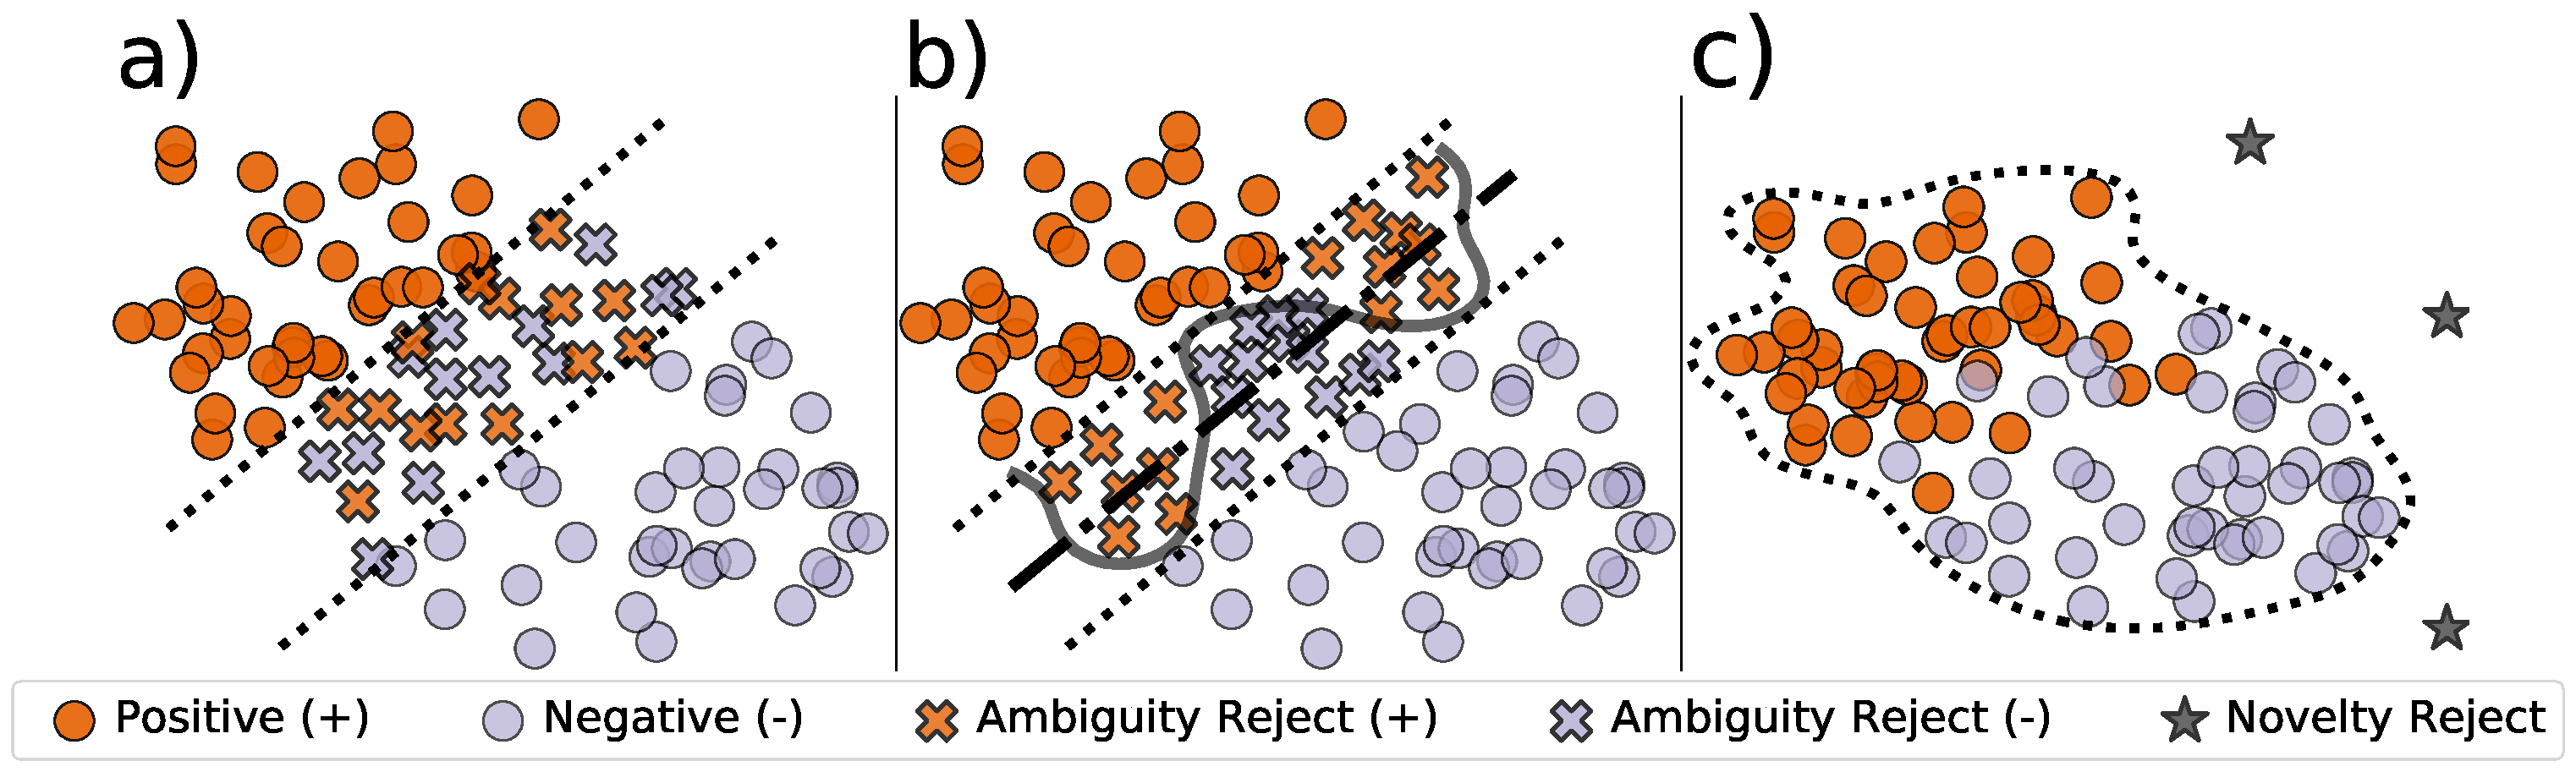
\includegraphics[width=\linewidth]{reject_classif2.pdf}
\caption{Illustration of a classification scenario where the two classes overlap in a region. The dotted lines represent the rejector, the dash-dotted line the fitted predictor $h$, and the solid line the ground truth relation $f$. a) shows ambiguity rejection due to a non-deterministic relation between $X$ and $Y$, b) introduces ambiguity rejection due to the model bias, and c) illustrates an example of novelty rejection. While in the first two plots the rejection region is inside the two dotted lines (examples with cross marks are rejected), in the third figure the rejected novel examples (stars) are outside the dotted line.
}
\label{fig:exampleclass2}
\end{figure}

\begin{figure}
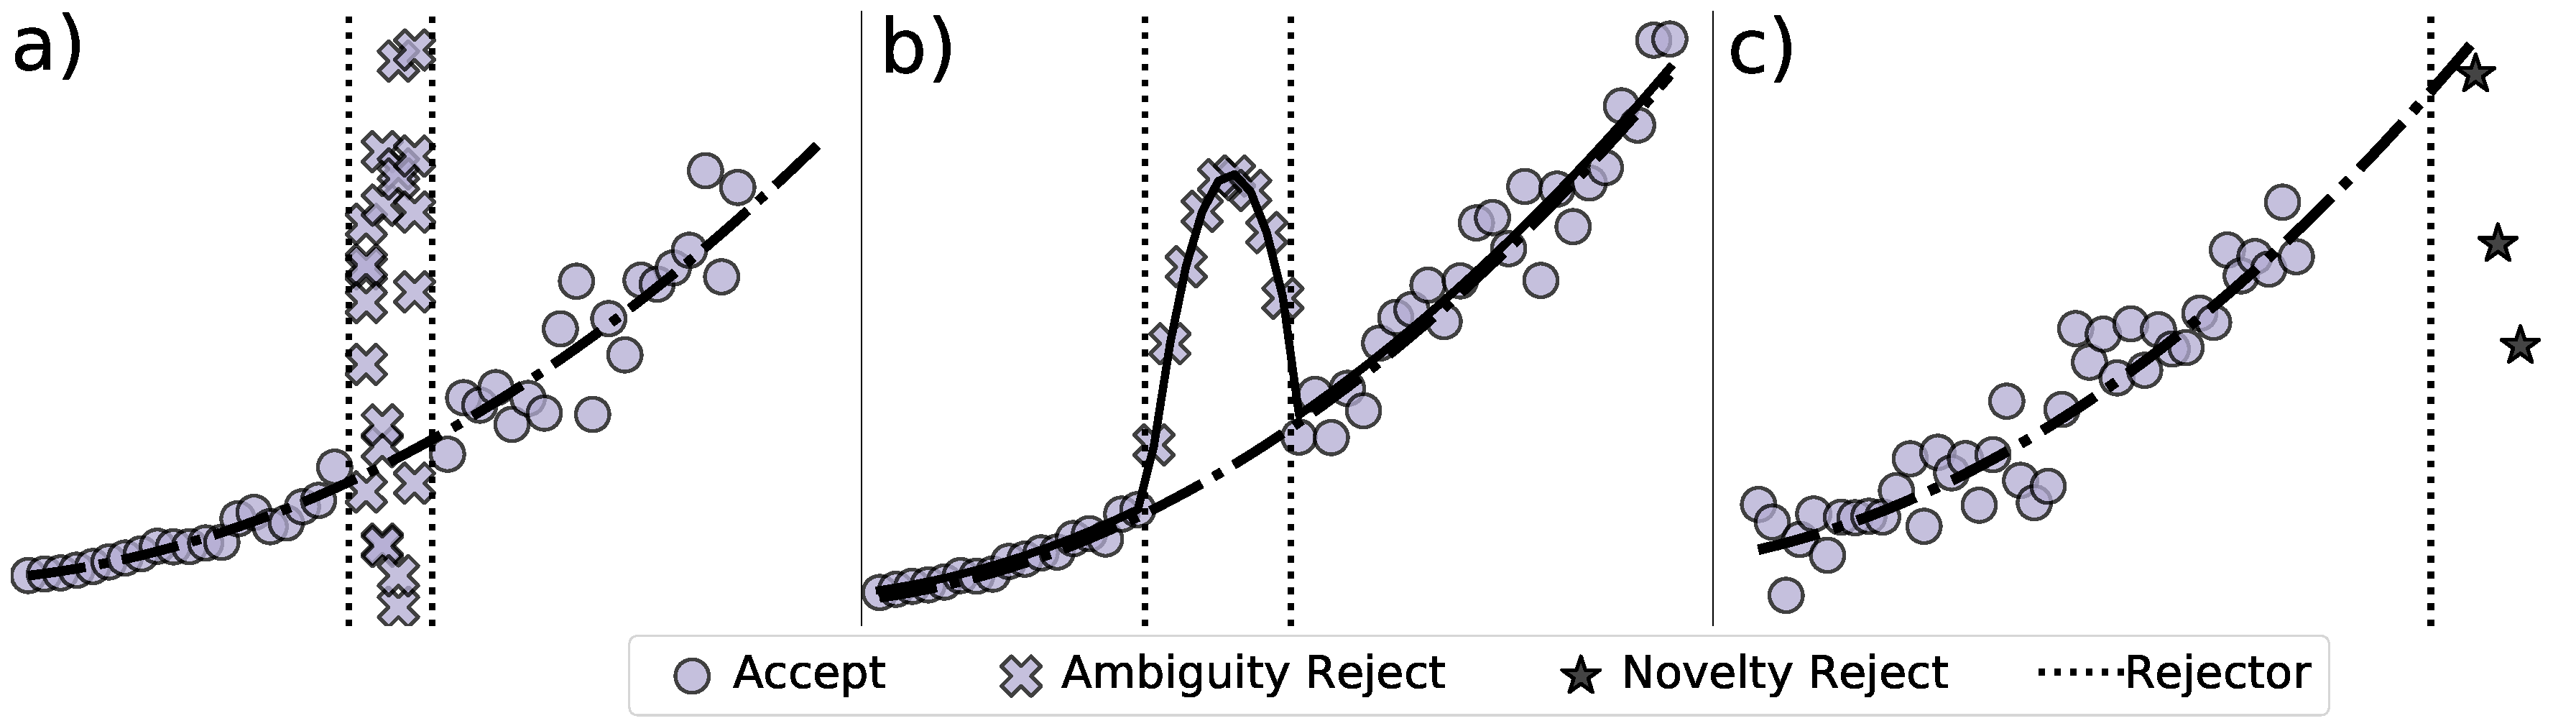
\includegraphics[width=\linewidth]{reject_regression.pdf}
\caption{Illustration of a regression scenario where rejection can be applied. The dash-dotted line represents the predictor $h$, while the solid line indicates the true function $f$. In a), examples in between the dotted lines are rejected (cross mark) due to the high variance of $Y$. In b), examples indicated with the cross mark are rejected due to the incorrect model bias. In c), star-marked examples are rejected because they differ from the training data (novelties).
}
\label{fig:examplereg2}
\end{figure}%

\begin{figure}
    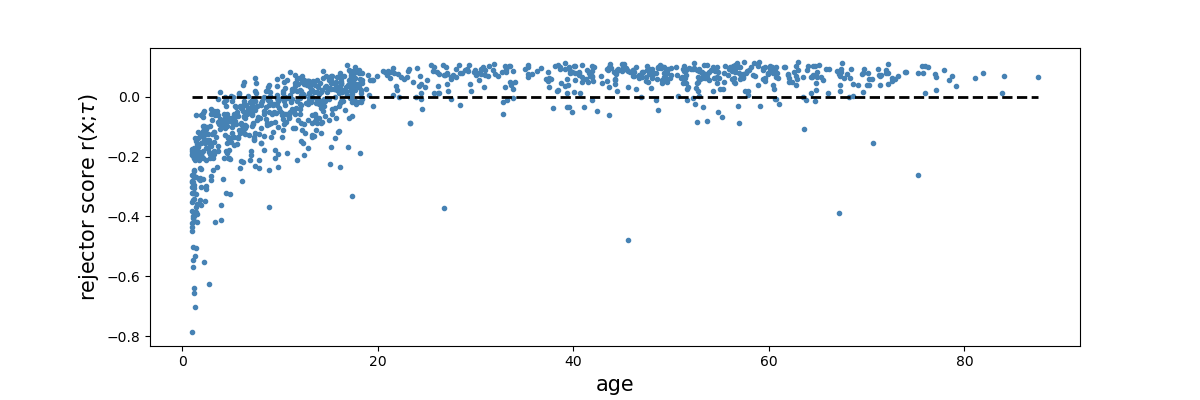
\includegraphics[width=\textwidth]{example_sleep_2.png}
    \caption{Results of a novelty reject option in a sleep stage scoring application \citep{VanderPlas2021}. The predictor is trained only on adults. The accuracy on children ($66.8\%$) is much lower than the accuracy on adults ($77.7\%$). Introducing the reject option mitigates the risk of making incorrect predictions as it ends up rejecting the predictions for most children.}
    \label{fig:sleep_example}
\end{figure}
